% Work/MAT, 1. ročník, 63. hodina – navazuje na hodiny 59–62.
% Primární podklad: ucebnice/02_Funkce_a_rovnice/Linearni_funkce_a_rovnice/Lineární funkce.tex
% Metodická inspirace: Realisticky.cz 020109–020110 (parametry a grafy přímek).
% Zadání, formulace a schémata vytvořena pro tuto přípravu; nikoli přepis externích úloh.
\documentclass[11pt,a4paper]{article}
\input{../../sablony/pripravy/priprava.sty}
\usepackage{tikz}
\usetikzlibrary{arrows.meta}
\nastavPripravu{1. ročník}{Funkce}{63}{Lineární funkce a její parametry}
\begin{document}
\poznamka{Povinné jádro na 45 minut: motivace 4 min, definice a graf 8 min, parametr $b$ 7 min,
parametr $a$ a odvození směrnice 10 min, vedený příklad 7 min, samostatný pokus a kontrola 7 min,
organizace 2 min. Další příklady a geometrické porovnávání patří do rezervy. Hodina 64 je samostatné procvičení.}

\blok{Od obecných funkcí k přímce}
V hodinách 59–62 jsme poznali funkci, definiční obor, obor hodnot, monotónnost a další vlastnosti.
Teď se zaměříme na funkci, jejíž hodnoty se při \emph{stejné změně argumentu} mění vždy o
\emph{stejný přírůstek}. Například $f(x)=2x+1$ dává pro argumenty $0,1,2,3$ hodnoty
$1,3,5,7$. Když zvýšíme $x$ o jednu jednotku, hodnota se vždy zvýší o dvě.

\begin{definiceBox}
\textbf{Lineární funkce} je funkce s definičním oborem $D(f)=\mathbb R$, kterou lze vyjádřit předpisem
\[
  f(x)=ax+b,\qquad a,b\in\mathbb R.
\]
Čísla $a,b$ jsou \textbf{parametry (koeficienty)} lineární funkce.
Jejím grafem je přímka. Pro $a=0$ dostáváme zvláštní případ: konstantní funkci.
\end{definiceBox}

Pokud zadání omezí obor, například $x\in\langle-1;2\rangle$, kreslíme jen odpovídající
\emph{část} přímky. Definice výše se týká funkce na celé $\mathbb R$.

\begin{center}
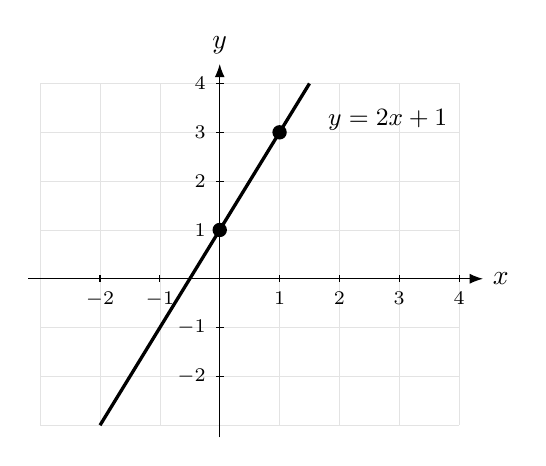
\begin{tikzpicture}[x=.76cm,y=.62cm,>=Latex]
\draw[step=1,gray!22,very thin] (-3,-3) grid (4,4);
\draw[->] (-3.2,0)--(4.4,0) node[right] {$x$};
\draw[->] (0,-3.25)--(0,4.4) node[above] {$y$};
\foreach \x in {-2,-1,1,2,3,4}{\draw (\x,.07)--(\x,-.07) node[below,font=\scriptsize] {$\x$};}
\foreach \y in {-2,-1,1,2,3,4}{\draw (.07,\y)--(-.07,\y) node[left,font=\scriptsize] {$\y$};}
\draw[very thick] (-2,-3)--(1.5,4);
\fill (0,1) circle (2.6pt);\fill (1,3) circle (2.6pt);
\node[anchor=west,font=\small] at (1.65,3.25) {$y=2x+1$};
\end{tikzpicture}
\end{center}
Přímka prochází například body $[0;1]$ a $[1;3]$. Dva \emph{různé} body ji určují;
třetí bod je vhodný pro kontrolu přesnosti konstrukce.

\blok{Parametr $b$: hodnota v nule}
\begin{definiceBox}
Číslo $b$ v předpisu $f(x)=ax+b$ je \textbf{absolutní člen}. Je-li $D(f)=\mathbb R$,
platí $f(0)=b$, a proto graf protíná osu $y$ v bodě $[0;b]$.
\end{definiceBox}
Porovnejme $f(x)=x$, $g(x)=x+2$ a $h(x)=x-1$. Všechny mají stejný sklon;
změnou $b$ jejich grafy \emph{svisle posouváme}. Přičtení $2$ posune celý graf o dvě jednotky nahoru.

\blok{Parametr $a$: směrnice a monotonie}
\begin{definiceBox}
Číslo $a$ v předpisu $f(x)=ax+b$ je \textbf{směrnice přímky}. Pro libovolná
$x_1\ne x_2$ platí
\[
 a=\frac{f(x_2)-f(x_1)}{x_2-x_1}=\frac{\Delta y}{\Delta x}.
\]
Vyjadřuje změnu funkční hodnoty při změně argumentu o jednotku.
\end{definiceBox}
Odvození z předpisu (nepoužíváme dosazení pouze dvou zvláštních hodnot):
\[
\frac{f(x_2)-f(x_1)}{x_2-x_1}
=\frac{(ax_2+b)-(ax_1+b)}{x_2-x_1}
=\frac{a(x_2-x_1)}{x_2-x_1}=a.
\]
Pro $a>0$ funkce roste, pro $a<0$ klesá a pro $a=0$ je konstantní.
Čím je $|a|$ větší, tím je přímka strmější (při stejném měřítku os).

\begin{center}
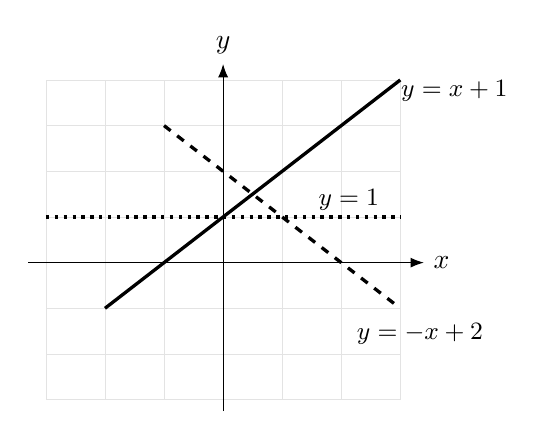
\begin{tikzpicture}[x=.75cm,y=.58cm,>=Latex]
\draw[step=1,gray!22,very thin] (-3,-3) grid (3,4);
\draw[->] (-3.3,0)--(3.4,0) node[right] {$x$};
\draw[->] (0,-3.25)--(0,4.35) node[above] {$y$};
\draw[very thick] (-2,-1)--(3,4);
\draw[very thick,dashed] (-1,3)--(3,-1);
\draw[very thick,dotted] (-3,1)--(3,1);
\node[font=\small,anchor=west] at (2.85,3.75) {$y=x+1$};
\node[font=\small,anchor=west] at (2.1,-1.55) {$y=-x+2$};
\node[font=\small,anchor=west] at (1.45,1.38) {$y=1$};
\end{tikzpicture}
\end{center}
\poznamka{Přímku s $a=0$ jen ukaž jako zvláštní případ. Samostatně ji s využitím slovní úlohy
probereme v hodinách 65–66. Zaměř se na přírůstky, ne na memorování „vpravo nahoru“.}

\blok{Řešené příklady}
\begin{prikladReseniBox}[title={Příklad 1: předpis, body a změna}]
Pro $f(x)=-2x+3$ určete $a$, $b$, dva body grafu a změnu funkční hodnoty při $\Delta x=3$.
\tcblower
$a=-2$, $b=3$, tedy graf prochází $[0;3]$. Pro $x=1$ je $f(1)=1$, druhý bod je $[1;1]$.
Protože $\Delta y=a\,\Delta x=-2\cdot3=-6$, při zvětšení argumentu o tři se hodnota
zmenší o šest. Funkce je klesající a na $\mathbb R$ prostá.
\end{prikladReseniBox}
\begin{prikladReseniBox}[title={Příklad 2: od dvou bodů k předpisu}]
Určete předpis lineární funkce procházející body $A[-1;4]$ a $B[2;-2]$.
\tcblower
\[
 a=\frac{-2-4}{2-(-1)}=\frac{-6}{3}=-2.
\]
Z bodu $A$ dostaneme $4=-2(-1)+b$, tedy $b=2$.
Hledaný předpis je $f(x)=-2x+2$. Kontrola: $f(2)=-2$.
\end{prikladReseniBox}

\blok{Samostatné procvičení}
\begin{zadaniReseniBox}[title={Krátká kontrola porozumění}]
\begin{enumerate}[label=\alph*)]
\item Urči $a,b$ a monotonii funkce $u(x)=\tfrac12 x-3$.
\item Proč jsou grafy $p(x)=3x-1$ a $q(x)=3x+2$ rovnoběžné? Který leží výše?
\item Urči předpis lineární funkce procházející body $[0;-2]$ a $[2;4]$.
\end{enumerate}
\tcblower
\begin{enumerate}[label=\alph*)]
\item $a=\frac12$, $b=-3$, funkce je rostoucí.
\item Směrnice obou je $3$; $q(x)-p(x)=3$, tedy $q$ leží o tři jednotky výše.
\item $b=-2$, $a=\frac{4-(-2)}{2-0}=3$, tedy $f(x)=3x-2$.
\end{enumerate}
\end{zadaniReseniBox}

\blok{Domácí úkol}
\begin{zadaniReseniBox}[title={Domácí procvičení}]
\begin{enumerate}[label=\alph*)]
\item U $f(x)=4-3x$ určete směrnici, absolutní člen, monotonii a $f(-2)$.
\item Vypočtěte předpis přímky procházející body $A[1;5]$, $B[3;9]$.
\item Jak souvisejí grafy $y=-2x+1$ a $y=-2x-4$? Vysvětlete bez rýsování.
\item Rozhodněte, zda je $u(x)=2x+1$ prostá a zda je sudá či lichá na $\mathbb R$.
\end{enumerate}
\tcblower
\begin{enumerate}[label=\alph*)]
\item $a=-3$, $b=4$, klesající, $f(-2)=10$.
\item $a=(9-5)/(3-1)=2$, $b=3$, tedy $f(x)=2x+3$.
\item Stejná směrnice $-2$, rovnoběžné; druhá přímka leží o pět jednotek níže.
\item Prostá je (směrnice $2\ne0$). Není sudá: $u(-x)=-2x+1\ne u(x)$;
není lichá: $u(-x)\ne-u(x)$ pro obecné $x$.
\end{enumerate}
\end{zadaniReseniBox}
\poznamka{Na 64. hodinu připrav pracovní list a pravítka. Vhodné je nechat studenty
první úlohu rýsovat ihned po výpočtu jejích bodů, ne všechny předpisy najednou.}
\end{document}
